\documentclass[10pt]{beamer}

% ------------------------------------------------------------------------
% Carga de tu preámbulo personalizado (preamble.tex)
% Asegúrate de tenerlo en la misma carpeta para que \input funcione.
% ------------------------------------------------------------------------
\usetheme[progressbar=frametitle]{metropolis}
\usepackage{appendixnumberbeamer}
\usepackage{fancyvrb}
\usepackage{booktabs}
\usepackage[scale=2]{ccicons}
\usepackage{pgfplots}
\usepgfplotslibrary{dateplot}
\usepackage{type1cm}
\usepackage{lettrine}
\usepackage{ragged2e}
\usepackage{xspace}
\newcommand{\themename}{\textbf{\textsc{metropolis}}\xspace}
\usepackage{graphicx} % Allows including images
\usepackage{booktabs} % Allows the use of \toprule, \midrule and \bottomrule in tables
\usepackage[utf8]{inputenc} %solucion del problema de los acentos.
\usepackage{xcolor}
\definecolor{LightGray}{gray}{0.9}

\usepackage{minted}
\usemintedstyle{tango}
\newcommand{\mypyfile}[1]{\inputminted[linenos=true, fontsize=\footnotesize, frame=lines, framesep=5\fboxrule,framerule=1pt]{python}{#1}}

\setminted[python]{breaklines,frame=lines,framesep=2mm,baselinestretch=1.2,bgcolor=LightGray,linenos, fontsize=\footnotesize} % obeytabs=true, tabsize=2, showtabs=true}

%%%%%%%%%%%%%%%%%%%%%%%%%%%%%%%%%%%%%%%%%%%%%%%%%%%%%%%%%%%%%%%%%%%%%%%%%%%%%%%%%%%%%%
\setbeamercolor{progress bar}{fg=blue!50!black,bg=white!50!black}
\setbeamercolor{title separator}{fg=red!50!black,bg=white!50!black}
\setbeamercolor{frametitle}{fg=white!80!black,bg=red!50!black}
\title[PCFI161]{Programaci\'on para F\'isica y Astronom\'ia}
\subtitle{Departamento de Física.}

\newcommand{\myfront}{
\author[PCFI161]{Corodinadora: C Loyola \\ Profesoras/es C Loyola / C Femenías / Y Navarrete / C Ruiz}
\institute[UNAB]{Universidad Andrés Bello}
\date{Primer Semestre 2025}
}

\titlegraphic{%
  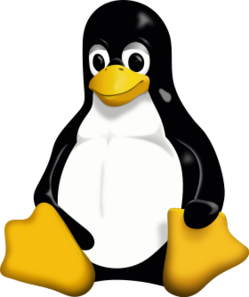
\includegraphics[width=.08\textwidth]{logo-tux.png}\hfill
  
\includegraphics[width=.3\textwidth]{logo-unab.png}\hfill
  
\includegraphics[width=.08\textwidth]{logo-python.png}
}

\makeatletter
\setbeamertemplate{title page}{
  \begin{minipage}[b][\paperheight]{\textwidth}
    \vfill%
    \ifx\inserttitle\@empty\else\usebeamertemplate*{title}\fi
    \ifx\insertsubtitle\@empty\else\usebeamertemplate*{subtitle}\fi
    \usebeamertemplate*{title separator}
    \ifx\beamer@shortauthor\@empty\else\usebeamertemplate*{author}\fi
    \ifx\insertdate\@empty\else\usebeamertemplate*{date}\fi
    \ifx\insertinstitute\@empty\else\usebeamertemplate*{institute}\fi
    \vfill
    \ifx\inserttitlegraphic\@empty\else\inserttitlegraphic\fi
    \vspace*{1cm}
  \end{minipage}
}
\makeatother


\makeatletter
\setlength{\metropolis@titleseparator@linewidth}{2pt}
\setlength{\metropolis@progressonsectionpage@linewidth}{2pt}
\setlength{\metropolis@progressinheadfoot@linewidth}{2pt}
\makeatother


\begin{document}

% ------------------------------------------------------------------------
% Portada personalizada (ejemplo \myfront si está definido en tu preámbulo)
% ------------------------------------------------------------------------
\myfront{}

% ------------------------------------------------------------------------
% Slide 1: Título de la Sesión
% ------------------------------------------------------------------------
\begin{frame}
  \titlepage
  % Por ejemplo:
  % \title{Semana 4 - Sesión 2 (Sesión 8): Taller de Funciones, Módulos y Librerías Externas}
\end{frame}

% ------------------------------------------------------------------------
% Slide 2: Índice / Tabla de Contenidos
% ------------------------------------------------------------------------
\begin{frame}
  \frametitle{Resumen - Semana 4, Sesión 2 (Sesión 8)}
  \tableofcontents
\end{frame}

% ------------------------------------------------------------------------
% Configuración de bloques
% ------------------------------------------------------------------------
\metroset{block=fill}

% ----------------------------------------------------------------------------------------
% SECCIÓN 1: Introducción y Repaso
% ----------------------------------------------------------------------------------------
\section{Introducción y Repaso}

% ------------------------------------------------------------------------
% Slide 3: Recapitulación de la Sesión 7
% ------------------------------------------------------------------------
\begin{frame}{Recapitulación de la Sesión Anterior (Sesión 7)}
  \begin{itemize}
    \item \textbf{Semana 4, Sesión 1 (Sesión 7)} se centró en:
      \begin{itemize}
        \item \textbf{Funciones}: sintaxis (\texttt{def}), parámetros, valores por defecto, alcance de variables.
        \item \textbf{Módulos y Paquetes}: cómo organizar el código en archivos \texttt{.py} y carpetas.
        \item Ejemplos de proyectos pequeños con \texttt{import} y definición de funciones útiles.
      \end{itemize}
    \item \textbf{Objetivo de hoy}: Ampliar la práctica con funciones y módulos, e \textbf{introducir el uso de librerías externas} (vía \texttt{pip} o Colab).
  \end{itemize}
\end{frame}

% ------------------------------------------------------------------------
% Slide 4: Objetivos de la Sesión 8
% ------------------------------------------------------------------------
\begin{frame}{Objetivos de la Sesión 8}
  \begin{itemize}
    \item \textbf{Profundizar} en el flujo de trabajo al crear y reutilizar módulos en Python.
    \item \textbf{Explorar} la instalación de librerías externas (\texttt{pip}, Google Colab).
    \item \textbf{Diseñar} una actividad grupal donde se combine la creación de funciones propias con el uso de librerías de terceros.
    \item \textbf{Fomentar} la colaboración y la discusión sobre buenas prácticas de organización.
  \end{itemize}
\end{frame}

% ----------------------------------------------------------------------------------------
% SECCIÓN 2: Repaso Rápido de Módulos y Paquetes
% ----------------------------------------------------------------------------------------
\section{Módulos y Paquetes (Repaso)}

% ------------------------------------------------------------------------
% Slide 5: Estructura de un Proyecto Simple
% ------------------------------------------------------------------------
\begin{frame}{Estructura Básica de un Proyecto}
  \begin{itemize}
    \item \textbf{Carpetas} y \texttt{.py} para agrupar funcionalidades.
    \item Ejemplo:
%\begin{verbatim}
%mi_proyecto/
%    main.py
%    mis_modulos/
%        __init__.py
%        matematicas.py
%        fisica.py
%\end{verbatim}
    \item \texttt{main.py} orquesta la lógica usando \texttt{import mis\_modulos.fisica} y así sucesivamente.
    \item Facilita la mantenibilidad y escalabilidad.
  \end{itemize}
\end{frame}

% ------------------------------------------------------------------------
% Slide 6: Importar vs. Desde
% ------------------------------------------------------------------------
\begin{frame}[fragile]{Formas de Importar}
\begin{itemize}
  \item \textbf{Import completo}:
  \begin{minted}{python}
import mis_modulos.matematicas
res = mis_modulos.matematicas.sumar(2, 3)
  \end{minted}
  \item \textbf{From / Import}:
  \begin{minted}{python}
from mis_modulos.matematicas import sumar
res = sumar(2, 3)
  \end{minted}
  \item \textbf{Import renombrado}:
  \begin{minted}{python}
import mis_modulos.matematicas as mm
res = mm.sumar(2, 3)
  \end{minted}
\end{itemize}
\end{frame}

% ----------------------------------------------------------------------------------------
% SECCIÓN 3: Librerías Externas y pip
% ----------------------------------------------------------------------------------------
\section{Librerías Externas}

% ------------------------------------------------------------------------
% Slide 7: ¿Por qué usar Librerías Externas?
% ------------------------------------------------------------------------
\begin{frame}{¿Por qué Librerías Externas?}
  \begin{itemize}
    \item \textbf{Ahorra tiempo}: aprovechas código ya probado por la comunidad.
    \item \textbf{Funcionalidades avanzadas}: Desde manejo de redes hasta machine learning.
    \item \textbf{Ejemplos}: \texttt{requests} para peticiones web, \texttt{numpy} para cálculo numérico, \texttt{pandas} para data frames, etc.
    \item \textbf{Comunidad activa}: librerías mantenidas, actualizaciones frecuentes.
  \end{itemize}
\end{frame}

% ------------------------------------------------------------------------
% Slide 8: Instalación con pip
% ------------------------------------------------------------------------
\begin{frame}[fragile]{Instalación con \texttt{pip}}
  \begin{itemize}
    \item \textbf{pip}: el gestor de paquetes oficial de Python.
    \item Comando general en terminal:
\begin{minted}{bash}
pip install nombre_paquete
\end{minted}
    \item Si usas \textbf{Google Colab}, puedes instalar temporalmente en una celda:
\begin{minted}{python}
!pip install nombre_paquete
\end{minted}
    \item La librería quedará disponible para importarse en el resto del entorno (hasta reiniciar).
  \end{itemize}
\end{frame}

% ------------------------------------------------------------------------
% Slide 9: Ejemplo: Instalando \texttt{requests} en Colab
% ------------------------------------------------------------------------
\begin{frame}[fragile]{Ejemplo: \texttt{requests} en Colab}
\begin{minted}{python}
# En una celda de Colab:
!pip install requests

import requests

resp = requests.get("https://api.github.com")
print(resp.status_code)
print(resp.json())
\end{minted}
\begin{itemize}
  \item \textbf{Uso real}: Conectarse a APIs, descargar datos, etc.
  \item \textbf{Sugerencia}: Manejar casos de error (\texttt{resp.status\_code != 200}).
\end{itemize}
\end{frame}

% ------------------------------------------------------------------------
% Slide 10: Ejemplo: Instalando \texttt{numpy}
% ------------------------------------------------------------------------
\begin{frame}[fragile]{Ejemplo: \texttt{numpy} Básico}
\begin{minted}{bash}
# Desde terminal local
pip install numpy
\end{minted}
\begin{minted}{python}
# Uso en el código
import numpy as np

arr = np.array([1, 2, 3, 4])
print(arr * 2)  # [2 4 6 8]
\end{minted}
\begin{itemize}
  \item \textbf{NumPy} es la base de muchas librerías científicas en Python.
  \item \textbf{Operaciones vectorizadas}: eficiencia y simplicidad.
\end{itemize}
\end{frame}

% ----------------------------------------------------------------------------------------
% SECCIÓN 4: Actividad Práctica
% ----------------------------------------------------------------------------------------
\section{Tarea Semanal}

% ------------------------------------------------------------------------
% Slide 11: Actividad: Creando un Módulo y Usando Librerías Externas
% ------------------------------------------------------------------------
\begin{frame}{Actividad General}
\begin{center}
  \huge{Manos a la Obra!}
\end{center}
\end{frame}


\begin{comment}

% ------------------------------------------------------------------------
% Slide 12: Lineamientos
% ------------------------------------------------------------------------
\begin{frame}{Lineamientos de la Actividad}
  \begin{itemize}
    \item Crear en Colab o localmente la siguiente estructura:
    
      \texttt{taller4/}\\
      \quad \texttt{mi\_modulo.py}\\
      \quad \texttt{main.ipynb} \quad \text{(o main.py)}\\
    
    \item \textbf{mi\_modulo.py}:
      \begin{itemize}
        \item Define algunas funciones (e.g., \texttt{multiplicar\_vector(vec, escalar)}) que internamente use \texttt{numpy}.
        \item Podrías incluir una función que calcule la \textbf{media} y \textbf{desviación estándar} de un arreglo con \texttt{numpy}.
      \end{itemize}
    \item \textbf{main.ipynb}:
      \begin{itemize}
        \item Instala (si es necesario) la librería \texttt{numpy}.
        \item Importa \texttt{mi\_modulo} y ejecuta las funciones, imprimiendo resultados.
      \end{itemize}
  \end{itemize}
\end{frame}

% ------------------------------------------------------------------------
% Slide 13: Ejemplo de \texttt{mi\_modulo.py}
% ------------------------------------------------------------------------
\begin{frame}[fragile]{Ejemplo: \texttt{mi\_modulo.py}}
\begin{minted}[fontsize=\tiny]{python}
import numpy as np

def multiplicar_vector(vec, escalar):
    """
    Multiplica cada elemento de 'vec' por 'escalar'.
    'vec' y 'escalar' pueden ser float o int.
    Retorna un np.array con el resultado.
    """
    arr = np.array(vec, dtype=float)
    return arr * escalar

def estadistica_basica(vec):
    """
    Retorna (media, desviacion_std) de vec,
    asumiendo que vec es convertible a np.array.
    """
    arr = np.array(vec, dtype=float)
    media = np.mean(arr)
    desv = np.std(arr)
    return (media, desv)
\end{minted}
\end{frame}

% ------------------------------------------------------------------------
% Slide 14: Ejemplo de \texttt{main.ipynb}
% ------------------------------------------------------------------------
\begin{frame}[fragile]{Ejemplo: \texttt{main.ipynb}}
\begin{minted}{python}
# En una celda:
!pip install numpy

# En otra celda:
import mi_modulo

resultado = mi_modulo.multiplicar_vector([1,2,3], 3)
print(f'Multiplicación: {resultado}')

media, desv = mi_modulo.estadistica_basica([10, 14, 22, 9])
print(f'Media = {media}, Desviación = {desv}')
\end{minted}
\begin{itemize}
  \item Observa cómo combinamos \textbf{nuestro módulo} con \textbf{numpy}.
  \item Podrías extender con más funciones o ejemplos.
\end{itemize}
\end{frame}

% ------------------------------------------------------------------------
% Slide 15: Trabajo en Grupos
% ------------------------------------------------------------------------
\begin{frame}{Trabajo en Grupos}
  \begin{itemize}
    \item Forma \textbf{parejas o tríos}.
    \item Diseña un \textbf{mini-proyecto} (inspirado en ejemplos de Física, Matemática, Astronomía, etc.).
    \item Usa \textbf{módulos propios} y una \textbf{librería externa} de tu elección (p.e. \texttt{requests} para datos en línea, \texttt{numpy} para vectores, \texttt{matplotlib} para graficar).
    \item Documenta brevemente cada función en \texttt{docstrings}.
  \end{itemize}
\end{frame}

% ------------------------------------------------------------------------
% Slide 16: Sugerencias
% ------------------------------------------------------------------------
\begin{frame}{Sugerencias para tu Mini-Proyecto}
  \begin{itemize}
    \item \textbf{Tema de Datos}: Descarga datos de Internet (por ejemplo, una tabla CSV) y analiza con \texttt{numpy}.
    \item \textbf{Tema de Física}: Define funciones de ecuaciones de movimiento y gráficas con \texttt{matplotlib}.
    \item \textbf{Tema Estadístico}: Genera datos aleatorios con \texttt{numpy} y calcula percentiles, histogramas, etc.
    \item \textbf{Pruebas y Validaciones}: Maneja entradas no válidas y verifica resultados esperados.
  \end{itemize}
\end{frame}

% ------------------------------------------------------------------------
% Slide 17: Tiempo de Desarrollo
% ------------------------------------------------------------------------
\begin{frame}{Tiempo de Desarrollo}
  \begin{itemize}
    \item Dedicar \textbf{20-30 minutos} a la construcción y prueba de los módulos.
    \item Intercambiar ideas y soluciones con el equipo.
    \item \textbf{Objetivo}: Tener un prototipo funcional que demuestre la unión de:
      \begin{itemize}
        \item Funciones personalizadas (en un módulo).
        \item Librería externa (instalada vía \texttt{pip} si hace falta).
      \end{itemize}
  \end{itemize}
\end{frame}

% ------------------------------------------------------------------------
% Slide 18: Espacio para Preguntas
% ------------------------------------------------------------------------
\begin{frame}{Espacio para Preguntas o Bloqueos}
  \begin{itemize}
    \item ¿Problemas al importar tu módulo (\texttt{ModuleNotFoundError})?
    \item ¿Incompatibilidad en Colab vs entorno local?
    \item ¿Dificultades con la instalación de librerías?
  \end{itemize}
  \vspace{0.2cm}
  \textbf{Comparte tu experiencia con el resto de la clase.}
\end{frame}

% ------------------------------------------------------------------------
% Slide 19: Comparte tu Solución
% ------------------------------------------------------------------------
\begin{frame}{Comparte tu Solución}
  \begin{itemize}
    \item Al cabo del tiempo de desarrollo:
      \begin{itemize}
        \item Muestra tu \textbf{código} y \textbf{resultados} a otros grupos.
        \item Explica brevemente la \textbf{arquitectura} (\texttt{mi\_modulo.py}, \texttt{main.ipynb}, etc.).
      \end{itemize}
    \item \textbf{Discutir}:
      \begin{itemize}
        \item ¿Qué librería externa se eligió y por qué?
        \item ¿Qué partes fueron más complejas?
      \end{itemize}
  \end{itemize}
\end{frame}

% ------------------------------------------------------------------------
% Slide 20: Ejemplo de Discusión
% ------------------------------------------------------------------------
\begin{frame}{Ejemplo de Discusión}
  \begin{block}{Grupo 1}
    \begin{itemize}
      \item Usó \texttt{numpy} para multiplicar matrices.
      \item Implementó una función \texttt{inversa\_matriz(A)} que devuelve \(\mathbf{A}^{-1}\).
    \end{itemize}
  \end{block}
  \vspace{0.4cm}
  \begin{block}{Grupo 2}
    \begin{itemize}
      \item Usó \texttt{requests} para descargar una tabla de datos climáticos en \texttt{CSV}.
      \item Creó una función para calcular la temperatura promedio y la humedad relativa.
    \end{itemize}
  \end{block}
\end{frame}

% ----------------------------------------------------------------------------------------
% SECCIÓN 5: Conclusiones
% ----------------------------------------------------------------------------------------
\section{Conclusiones y Próximos Pasos}

% ------------------------------------------------------------------------
% Slide 21: Análisis General
% ------------------------------------------------------------------------
\begin{frame}{Análisis General de la Actividad}
  \begin{itemize}
    \item Ventajas de \textbf{combinar módulos propios con librerías externas}:
      \begin{itemize}
        \item Reutilización de código (módulos).
        \item Potencia y robustez (librerías de terceros).
      \end{itemize}
    \item Importancia de la \textbf{organización de archivos} y de un \textbf{flujo de trabajo} claro.
    \item Manejar \textbf{entornos virtuales} (en local) es otra buena práctica (tema futuro).
  \end{itemize}
\end{frame}

% ------------------------------------------------------------------------
% Slide 22: Recomendaciones de Estudio
% ------------------------------------------------------------------------
\begin{frame}{Recomendaciones de Estudio}
  \begin{itemize}
    \item Revisar la \textbf{documentación oficial} de \texttt{pip} y \texttt{virtualenv}.
    \item Explorar \textbf{PyPI} (\url{https://pypi.org/}) para descubrir librerías útiles.
    \item Practicar la creación de \textbf{módulos} en proyectos pequeños.
    \item Investigar qué librerías podrían ser útiles para futuros trabajos de Física/Astronomía (p.e. \texttt{astropy}, \texttt{scipy}).
  \end{itemize}
\end{frame}


\end{comment}

% ------------------------------------------------------------------------
% Slide 23: Visión de la Próxima Sesión
% ------------------------------------------------------------------------
\begin{frame}{Próxima Sesión}
  \begin{itemize}
    \item \textbf{Sesion 9 (Semana 5)}: Repaso integral de Unidades I y II, y \textbf{Solemne I}.
    \item \textbf{Recomendación}:
      \begin{itemize}
        \item Revisa todos los conceptos vistos: Sintaxis, Estructuras de Control, Funciones, Módulos.
        \item Práctica con ejercicios y ejemplos de exámenes pasados (si los hubiera).
      \end{itemize}
  \end{itemize}
  \vspace{0.3cm}
  \textbf{¡Prepárate para la evaluación!}
\end{frame}

% ------------------------------------------------------------------------
% Slide 24: Recursos Adicionales
% ------------------------------------------------------------------------
\begin{frame}{Recursos Adicionales}
  \begin{itemize}
    \item \href{https://packaging.python.org/tutorials/installing-packages/}{\textbf{Official Python Packaging Tutorial}}
    \item \href{https://docs.python.org/3/library/}{\textbf{Documentación de la Biblioteca Estándar de Python}}
    \item \href{https://pypi.org/}{\textbf{PyPI}} - Python Package Index
    \item \href{https://numpy.org/doc/}{\textbf{Numpy Docs}}
    \item \href{https://matplotlib.org/stable/}{\textbf{Matplotlib Docs}}
  \end{itemize}
\end{frame}

% ------------------------------------------------------------------------
% Slide 25: Cierre de la Sesión
% ------------------------------------------------------------------------
\begin{frame}
  \huge{\centerline{¡Muchas gracias y éxito en su práctica!}}
  \vspace{0.4cm}
  \normalsize
  \begin{itemize}
    \item Recuerden subir su trabajo a Google Drive o repositorio compartido.
    \item Próxima sesión: \textbf{Solemne I} y repaso integral.
    \item ¡Sigan explorando librerías externas y creando módulos propios!
  \end{itemize}
\end{frame}

\end{document}

